\chapter*{Introduction}
\label{chap:Introduction}
\renewcommand{\thesection}{\arabic{section}}
\setcounter{section}{0}

Through my partner, who is a physiotherapist, I get some insights into the medicinal field and medicinal devices which are used. Some of these devices are equipped with simple sensors and still cost a fortune. This shocked me but also sparked my interest. Products which she encountered are applied to improve gait and posture. Since Back pain is a very common issue ("reported lifetime prevalence ranges widely from 49\%-70\%" \cite{backpain00:study}) and can, in many cases, be traced back to a bad posture while seated \cite{sitting00:study}. I had the idea of creating an affordable device, which improves posture while sitting. I felt like this would offer a great benefit for others and also something myself could use.

Technical solutions to avoid bad posture already do exist. However, none of them seemed to be affordable, simple and open source. These products can be found in the section "Similar Products". Some of them are quite expensive (up to 10'000 CHF) others are obfuscated and closed source and some have a great concept, however are in a different area of application. Therefore I decided to try and create a simple and cheap device which can measure and improve posture. Additionally, it should all be open source and recreatable. Besides posture, the goal is to also offer a way to improve balance, which might one day be applied by physiotherapists.
With the idea of improving balance also comes a much larger goal which might not even be achievable. The solutions should be able to be applied in the medicinal field, however this seams to be nearly impossible due to the complexity and restrictions in this field. 

Before beginning the technical implementation it is very important to investigate what already exists on the market.



\section{Similar Devices}


Usually someone already had a similar idea, or something which tries to solve the same problems has already been produced. Therefore it is important to investigate similar devices and products. A few examples of such devices are described below.

\subsection{Sming}

\begin{wrapfigure}{R}{0.15\textwidth}
  \begin{center}
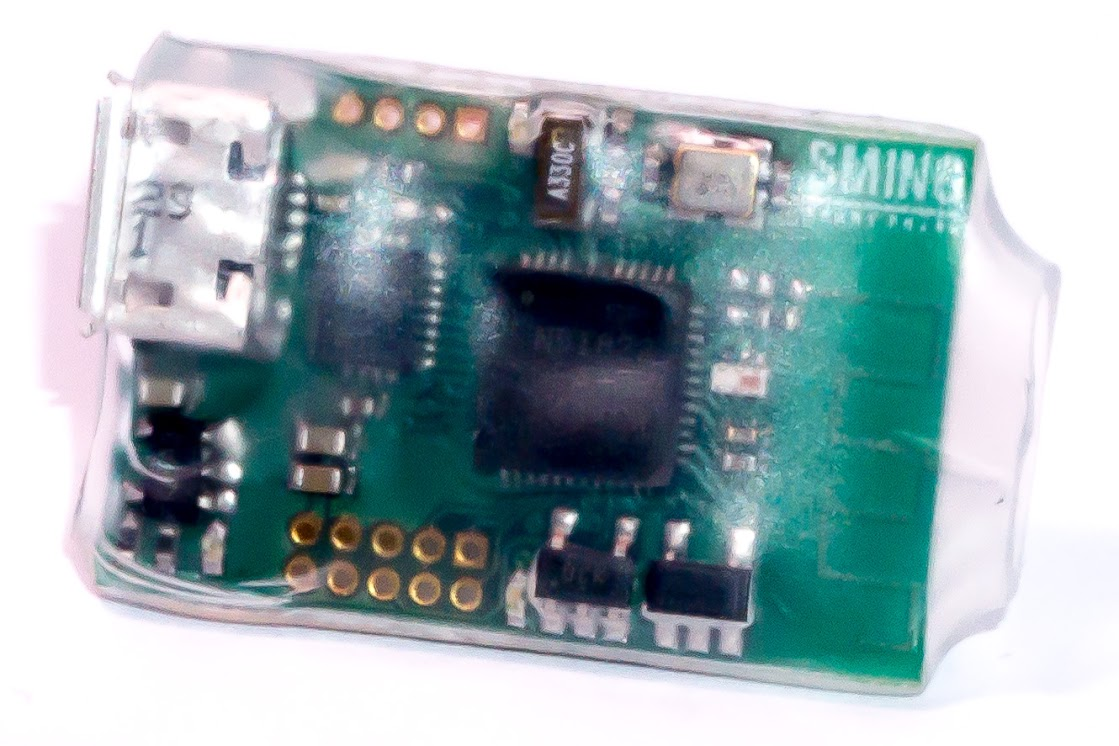
\includegraphics[width=\linewidth]{images/sming_pic2.jpg}
  \end{center}
  \caption{\label{fig:Sming}Sming \cite{sming:book}}
\end{wrapfigure}

The first similar product i would like to name is the "SMING". The Sming is a sensor node created with the BFH. 
It is using the Sensor "TXW51" which has an acceleromter and a gyroscope. This devices uses Bluetooth smart to communicate. It was created for a master thesis and is a great example of how small such a device can be. 

It was planned to use the device for sports measurement and was designed to very energy efficient. However according to my know-how the device never has been in use productively. \cite{sming:book}
Such a device and the know-how gathered for this projects might be a great starting point when designing a "all in one" sensor packet for my use case. "SMING" might offer a lot even when used as is. This will need to be evaluated in the near future.

\newpage
\subsection{Swaystar}

\begin{wrapfigure}{R}{0.15\textwidth}
 \vspace{-20pt}
  \begin{center}
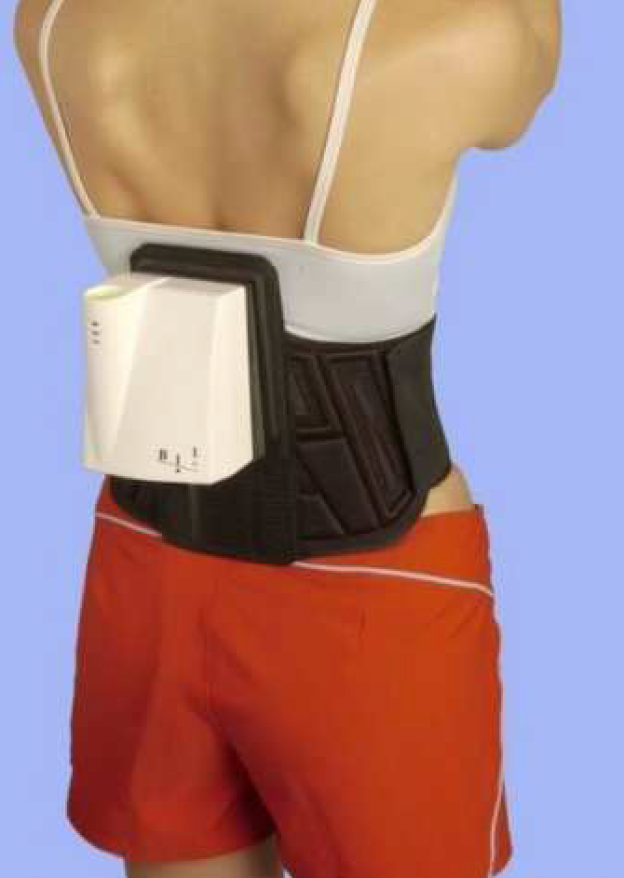
\includegraphics[width=\linewidth]{images/Swaystar_01.png}
  \end{center}
  \caption{\label{fig:swaystar}Swaystar}
\end{wrapfigure}

The following existing product was the trigger for my project idea. The so called swaystar \ref{fig:swaystar} offers almost the same functionality, however it is at least 10 times bigger and costs about 10'000 CHF. 
I have never used such a device, however i have talked to people who worked with one. Apparently it tracks the movement / positioning of users and stores the data. An additional headband can be purchased with which vibrations are sent to the user so he can improve his body ergonomics and balance. 

As said, it offers a very similar functionality, however not it covers the same use cases. Due to the size and price it can almost exclusively only be used in therapies and by medical professionals. My device intends to target the end user, and offer an easier and more affordable solution. The swaystar also is closed-source and appears to be a rather old product.
\cite{SwayStar47:online}

\subsection{Go Posture trainer}

\begin{wrapfigure}{r}{0.2\textwidth}
  \begin{center}
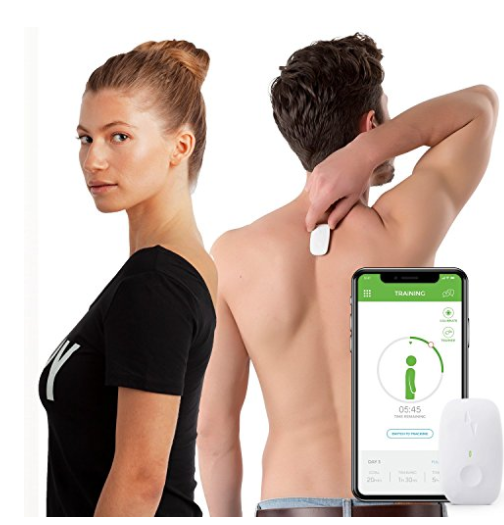
\includegraphics[width=\linewidth]{images/Screenshot_3.png}
  \end{center}
  \caption{Go Posture trainer}
  \label{fig:gotrainer}
\end{wrapfigure}

Further investigations into other products, were almost fruitless. There are some apps which offer almost the same thing I have tried to achieve with my app, but a bit more refined and there is one product which offers a use-case that could be considered equal to the first defined use-case (improved sitting posture), at least on first glance (\ref{fig:gotrainer} Go Trainer). 

The product functions as a posture trainer, it has to be attached to the back, and it is, even if small, quite visible under a shirt. Secondly the device only offers a mono-directional biofeedback. \cite{HowToImp2:online} The costs about 80\$ which I would consider affordable.

Furthermore the device is closed source and is only targeted to users who want to improve their posture. As mentioned the plan for my device would be to keep everything open-source and cover a wider range of use-cases. 

Other contraptions to improve posture use cloth to physically "pull" the user in the right position. This is an interesting concept and usually is quite cheap. Since it is a completely different approach, I would not consider these contraptions to be directly comparable.

After these investigations and also further investigations into the medical field I considered my device to still be an innovation, offering something which is not yet available on the market.